\documentclass[border=4pt,12pt]{standalone}
% House style for redrawn exam diagrams (diagram-v4: 0.4pt lines, filled -latex arrows, fine dashes; stipple and hatching drawn as real dots/lines (no PDF/SVG patterns, so they render in every browser and at any scale); transparent background). Every figure \input's this.
\usepackage{amsmath,amssymb}
\usepackage{txfonts}
\usepackage{pdfrender,xcolor}
% \halo{text}: label on shading. The shading stops just around each letter's outline (a thin knock-out that follows the
% glyphs, like the papers' typesetting), never a box. Owner: "I don't want a box around the text".
\newcommand{\halo}[1]{\leavevmode\rlap{\pdfrender{TextRenderingMode=2,LineWidth=2.2pt,LineJoinStyle=1,StrokeColor=white,FillColor=white}#1}#1}
\usepackage{tikz,pgfplots}
\pgfplotsset{compat=1.18}
\usetikzlibrary{arrows.meta,calc,angles,quotes,patterns,patterns.meta,intersections,positioning,decorations.markings,shapes.geometric}
% Stipple and hatching are drawn as actual dots / lines clipped to the region (path picture), NOT as pattern fills:
% SVG <pattern> fills vanish or blur when browsers scale the image, so the owner could not see the shading.
% Each dot is a 0.72pt square (keeps SVGs small; reads as a dot at print size). Dots sit on one global staggered grid, so neighbouring regions line up.
\makeatletter
\newdimen\ex@x \newdimen\ex@y \newdimen\ex@xa \newdimen\ex@ya \newdimen\ex@xb \newdimen\ex@yb \newcount\ex@row
\def\exam@stipplecolor{black!75}\def\exam@dotr{0.42pt}\def\exam@dotgap{2.5}
\def\ex@rowdots{\ifdim\ex@x<\ex@xb \pgfpathrectangle{\pgfqpoint{\dimexpr\ex@x-0.36pt\relax}{\dimexpr\ex@y-0.36pt\relax}}{\pgfqpoint{0.72pt}{0.72pt}}\advance\ex@x by \exam@dotgap pt\relax\expandafter\ex@rowdots\fi}
\def\exam@stipple{%
  \pgftransformreset% dots are sized in real points even inside scaled pictures
  \pgfpointanchor{path picture bounding box}{south west}\ex@xa=\pgf@x \ex@ya=\pgf@y
  \pgfpointanchor{path picture bounding box}{north east}\ex@xb=\pgf@x \ex@yb=\pgf@y
  \pgfsetfillcolor{\exam@stipplecolor}\pgfmathsetmacro\ex@h{\exam@dotgap/2}%
  \pgfmathtruncatemacro\ex@r{floor(\ex@ya/\ex@h)-1}\ex@row=\ex@r\relax
  \ex@y=\ex@r\dimexpr\ex@h pt\relax
  \loop\ifdim\ex@y<\ex@yb
    \pgfmathtruncatemacro\ex@c{floor(\ex@xa/\exam@dotgap)-1}\ex@x=\ex@c\dimexpr\exam@dotgap pt\relax
    \ifodd\ex@row \advance\ex@x by \ex@h pt\fi
    \ex@rowdots
    \advance\ex@y by \ex@h pt \advance\ex@row by 1
    \ifnum\numexpr\ex@row-(\ex@row/4)*4\relax=0 \pgfusepath{fill}\fi% flush every 4 rows: bounded TeX memory, few clip copies in the SVG
  \repeat\pgfusepath{fill}}
\newdimen\ex@d
\def\exam@hatch#1{% #1 = 1 for /, -1 for \ ; lines 45 degrees, 3pt apart
  \pgftransformreset
  \pgfpointanchor{path picture bounding box}{south west}\ex@xa=\pgf@x \ex@ya=\pgf@y
  \pgfpointanchor{path picture bounding box}{north east}\ex@xb=\pgf@x \ex@yb=\pgf@y
  \ex@d=\dimexpr\ex@yb-\ex@ya\relax \ex@x=\dimexpr\ex@xa-\ex@d\relax
  \loop\ifdim\ex@x<\ex@xb
    \ifnum#1>0 \pgfpathmoveto{\pgfqpoint{\ex@x}{\ex@ya}}\pgfpathlineto{\pgfqpoint{\dimexpr\ex@x+\ex@d\relax}{\ex@yb}}%
    \else \pgfpathmoveto{\pgfqpoint{\ex@x}{\ex@yb}}\pgfpathlineto{\pgfqpoint{\dimexpr\ex@x+\ex@d\relax}{\ex@ya}}\fi
    \advance\ex@x by 4.24pt
  \repeat
  \pgfsetlinewidth{0.4pt}\pgfsetstrokecolor{black}\pgfusepath{stroke}}
\def\examstipple{\exam@stipple}\def\examhatch{\exam@hatch}\def\examsetstipplecolor#1{\def\exam@stipplecolor{#1}}\def\examsetdotgap#1{\def\exam@dotgap{#1}}
\makeatother
% (legacy pattern kept for old files)
% staggered stipple like the NESA papers' dotted shading
\pgfdeclarepatternformonly{exam stipple}{\pgfpointorigin}{\pgfqpoint{2.2pt}{2.2pt}}{\pgfqpoint{2.2pt}{2.2pt}}{%
  \pgfpathcircle{\pgfqpoint{0.55pt}{0.55pt}}{0.42pt}\pgfpathcircle{\pgfqpoint{1.65pt}{1.65pt}}{0.42pt}\pgfusepath{fill}}
\tikzset{
  every picture/.style={line width=0.6pt, >={Latex[length=2mm,width=1.3mm]}},
  curve/.style={line width=0.6pt},
  open arrow/.style={-{Latex[length=2mm,width=1.3mm]}},  % owner: filled -latex heads everywhere, no open chevrons
  aux/.style={dash pattern=on 2pt off 1.5pt, line width=0.6pt},
  shade/.code={\def\exA{#1}\def\exB{none}\ifx\exA\exB\else\pgfkeysalso{fill=black!18}\fi},
  shade/.default=on,
  shade dots/.style={fill=none, path picture={\examstipple}},
  stipple color/.code={\examsetstipplecolor{#1}},
  stipple gap/.code={\examsetdotgap{#1}},
  shade dense dots/.style={fill=none, stipple gap=1.6, path picture={\examstipple}},
  shade hatch/.style={fill=none, path picture={\examhatch{1}}},
  shade hatch reverse/.style={fill=none, path picture={\examhatch{-1}}},
  shade solid/.style={fill=black},
  pt/.style={circle, fill, inner sep=1.1pt},
  open pt/.style={circle, draw, fill=white, inner sep=1.1pt},
}
\pgfplotsset{
  exam axes/.style={axis lines=middle, axis line style={->}, xlabel={$x$}, ylabel={$y$},
    xlabel style={anchor=west}, ylabel style={anchor=south}, tick label style={font=\small},
    every axis plot/.append style={line width=0.6pt, black}, samples=200, clip=false,
    enlargelimits=false, axis on top},
}

\begin{document}
% 2025 Penrith AT4 Q23 solution: f (grey: given part x>0 and its odd extension x<0) and h(x)=f(x/2)+2 (black), with asymptotes.
% Crop colours: grey/green = f, red = h. Curves traced from the crop and refitted smooth. (crop pixels, y down)
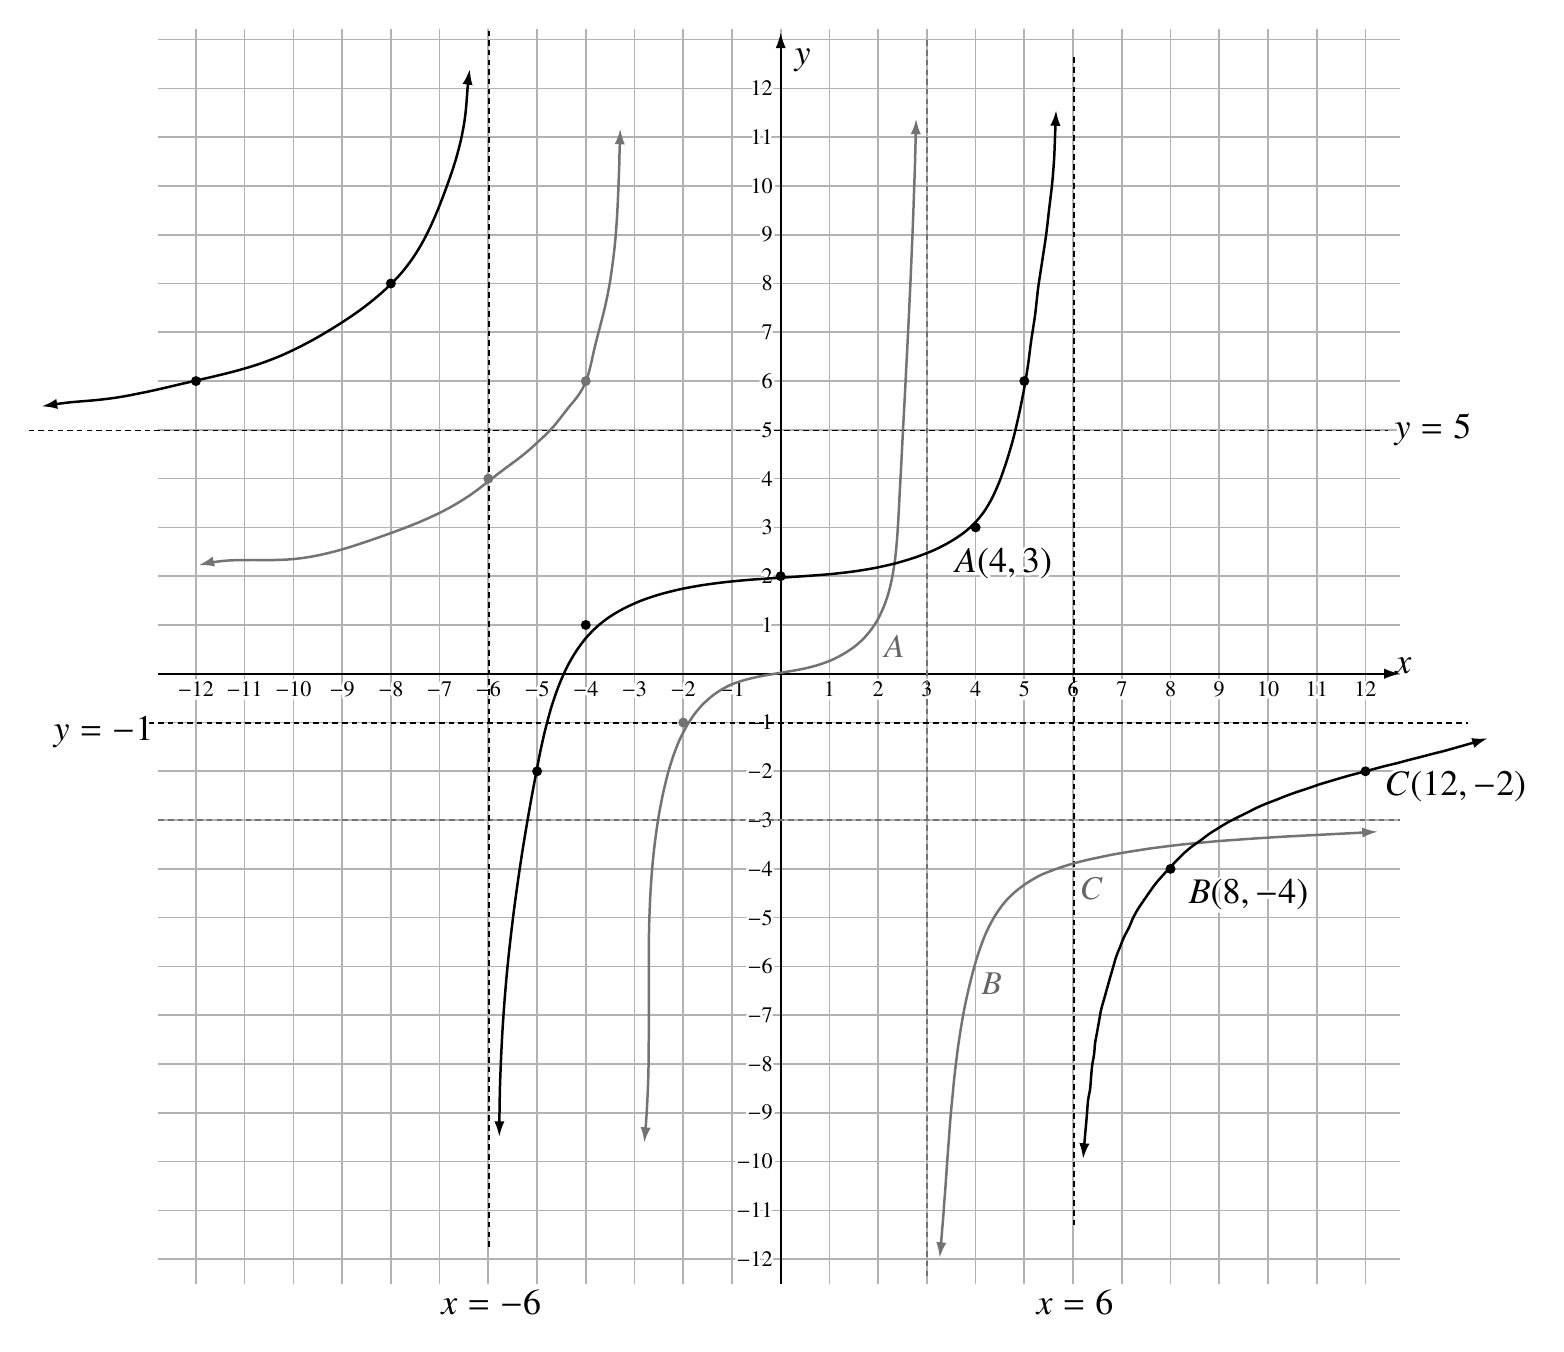
\begin{tikzpicture}[x=0.0127cm,y=-0.0127cm,font=\fontsize{8}{9.5}\selectfont]
  \draw[black!30] (167.5,6) -- (167.5,1262);
  \draw[black!30] (216.2,6) -- (216.2,1262);
  \draw[black!30] (265.0,6) -- (265.0,1262);
  \draw[black!30] (313.8,6) -- (313.8,1262);
  \draw[black!30] (362.5,6) -- (362.5,1262);
  \draw[black!30] (411.2,6) -- (411.2,1262);
  \draw[black!30] (460.0,6) -- (460.0,1262);
  \draw[black!30] (508.8,6) -- (508.8,1262);
  \draw[black!30] (557.5,6) -- (557.5,1262);
  \draw[black!30] (606.2,6) -- (606.2,1262);
  \draw[black!30] (655.0,6) -- (655.0,1262);
  \draw[black!30] (703.8,6) -- (703.8,1262);
  \draw[black!30] (752.5,6) -- (752.5,1262);
  \draw[black!30] (801.2,6) -- (801.2,1262);
  \draw[black!30] (850.0,6) -- (850.0,1262);
  \draw[black!30] (898.8,6) -- (898.8,1262);
  \draw[black!30] (947.5,6) -- (947.5,1262);
  \draw[black!30] (996.2,6) -- (996.2,1262);
  \draw[black!30] (1045.0,6) -- (1045.0,1262);
  \draw[black!30] (1093.8,6) -- (1093.8,1262);
  \draw[black!30] (1142.5,6) -- (1142.5,1262);
  \draw[black!30] (1191.2,6) -- (1191.2,1262);
  \draw[black!30] (1240.0,6) -- (1240.0,1262);
  \draw[black!30] (1288.8,6) -- (1288.8,1262);
  \draw[black!30] (1337.5,6) -- (1337.5,1262);
  \draw[black!30] (130,1237.1) -- (1372,1237.1);
  \draw[black!30] (130,1188.3) -- (1372,1188.3);
  \draw[black!30] (130,1139.5) -- (1372,1139.5);
  \draw[black!30] (130,1090.7) -- (1372,1090.7);
  \draw[black!30] (130,1041.9) -- (1372,1041.9);
  \draw[black!30] (130,993.1) -- (1372,993.1);
  \draw[black!30] (130,944.3) -- (1372,944.3);
  \draw[black!30] (130,895.5) -- (1372,895.5);
  \draw[black!30] (130,846.7) -- (1372,846.7);
  \draw[black!30] (130,797.9) -- (1372,797.9);
  \draw[black!30] (130,749.1) -- (1372,749.1);
  \draw[black!30] (130,700.3) -- (1372,700.3);
  \draw[black!30] (130,651.5) -- (1372,651.5);
  \draw[black!30] (130,602.7) -- (1372,602.7);
  \draw[black!30] (130,553.9) -- (1372,553.9);
  \draw[black!30] (130,505.1) -- (1372,505.1);
  \draw[black!30] (130,456.3) -- (1372,456.3);
  \draw[black!30] (130,407.5) -- (1372,407.5);
  \draw[black!30] (130,358.7) -- (1372,358.7);
  \draw[black!30] (130,309.9) -- (1372,309.9);
  \draw[black!30] (130,261.1) -- (1372,261.1);
  \draw[black!30] (130,212.3) -- (1372,212.3);
  \draw[black!30] (130,163.5) -- (1372,163.5);
  \draw[black!30] (130,114.7) -- (1372,114.7);
  \draw[black!30] (130,65.9) -- (1372,65.9);
  \draw[black!30] (130,17.1) -- (1372,17.1);
  \draw[->] (130,651.5) -- (1372,651.5);
  \draw[->] (752.5,1262) -- (752.5,10);
  \node[anchor=south west,inner sep=1pt,font=\fontsize{13}{15}\selectfont] at (1362,655) {$x$};
  \node[anchor=west,inner sep=2pt,font=\fontsize{13}{15}\selectfont] at (760,38) {$y$};
  \node[anchor=north,inner sep=1.5pt] at (167.5,654.5) {\halo{$-12$}};
  \node[anchor=north,inner sep=1.5pt] at (216.2,654.5) {\halo{$-11$}};
  \node[anchor=north,inner sep=1.5pt] at (265.0,654.5) {\halo{$-10$}};
  \node[anchor=north,inner sep=1.5pt] at (313.8,654.5) {\halo{$-9$}};
  \node[anchor=north,inner sep=1.5pt] at (362.5,654.5) {\halo{$-8$}};
  \node[anchor=north,inner sep=1.5pt] at (411.2,654.5) {\halo{$-7$}};
  \node[anchor=north,inner sep=1.5pt] at (460.0,654.5) {\halo{$-6$}};
  \node[anchor=north,inner sep=1.5pt] at (508.8,654.5) {\halo{$-5$}};
  \node[anchor=north,inner sep=1.5pt] at (557.5,654.5) {\halo{$-4$}};
  \node[anchor=north,inner sep=1.5pt] at (606.2,654.5) {\halo{$-3$}};
  \node[anchor=north,inner sep=1.5pt] at (655.0,654.5) {\halo{$-2$}};
  \node[anchor=north,inner sep=1.5pt] at (703.8,654.5) {\halo{$-1$}};
  \node[anchor=north,inner sep=1.5pt] at (801.2,654.5) {\halo{$1$}};
  \node[anchor=north,inner sep=1.5pt] at (850.0,654.5) {\halo{$2$}};
  \node[anchor=north,inner sep=1.5pt] at (898.8,654.5) {\halo{$3$}};
  \node[anchor=north,inner sep=1.5pt] at (947.5,654.5) {\halo{$4$}};
  \node[anchor=north,inner sep=1.5pt] at (996.2,654.5) {\halo{$5$}};
  \node[anchor=north,inner sep=1.5pt] at (1045.0,654.5) {\halo{$6$}};
  \node[anchor=north,inner sep=1.5pt] at (1093.8,654.5) {\halo{$7$}};
  \node[anchor=north,inner sep=1.5pt] at (1142.5,654.5) {\halo{$8$}};
  \node[anchor=north,inner sep=1.5pt] at (1191.2,654.5) {\halo{$9$}};
  \node[anchor=north,inner sep=1.5pt] at (1240.0,654.5) {\halo{$10$}};
  \node[anchor=north,inner sep=1.5pt] at (1288.8,654.5) {\halo{$11$}};
  \node[anchor=north,inner sep=1.5pt] at (1337.5,654.5) {\halo{$12$}};
  \node[anchor=east,inner sep=1.5pt] at (749.5,1237.1) {\halo{$-12$}};
  \node[anchor=east,inner sep=1.5pt] at (749.5,1188.3) {\halo{$-11$}};
  \node[anchor=east,inner sep=1.5pt] at (749.5,1139.5) {\halo{$-10$}};
  \node[anchor=east,inner sep=1.5pt] at (749.5,1090.7) {\halo{$-9$}};
  \node[anchor=east,inner sep=1.5pt] at (749.5,1041.9) {\halo{$-8$}};
  \node[anchor=east,inner sep=1.5pt] at (749.5,993.1) {\halo{$-7$}};
  \node[anchor=east,inner sep=1.5pt] at (749.5,944.3) {\halo{$-6$}};
  \node[anchor=east,inner sep=1.5pt] at (749.5,895.5) {\halo{$-5$}};
  \node[anchor=east,inner sep=1.5pt] at (749.5,846.7) {\halo{$-4$}};
  \node[anchor=east,inner sep=1.5pt] at (749.5,797.9) {\halo{$-3$}};
  \node[anchor=east,inner sep=1.5pt] at (749.5,749.1) {\halo{$-2$}};
  \node[anchor=east,inner sep=1.5pt] at (749.5,700.3) {\halo{$-1$}};
  \node[anchor=east,inner sep=1.5pt] at (749.5,602.7) {\halo{$1$}};
  \node[anchor=east,inner sep=1.5pt] at (749.5,553.9) {\halo{$2$}};
  \node[anchor=east,inner sep=1.5pt] at (749.5,505.1) {\halo{$3$}};
  \node[anchor=east,inner sep=1.5pt] at (749.5,456.3) {\halo{$4$}};
  \node[anchor=east,inner sep=1.5pt] at (749.5,407.5) {\halo{$5$}};
  \node[anchor=east,inner sep=1.5pt] at (749.5,358.7) {\halo{$6$}};
  \node[anchor=east,inner sep=1.5pt] at (749.5,309.9) {\halo{$7$}};
  \node[anchor=east,inner sep=1.5pt] at (749.5,261.1) {\halo{$8$}};
  \node[anchor=east,inner sep=1.5pt] at (749.5,212.3) {\halo{$9$}};
  \node[anchor=east,inner sep=1.5pt] at (749.5,163.5) {\halo{$10$}};
  \node[anchor=east,inner sep=1.5pt] at (749.5,114.7) {\halo{$11$}};
  \node[anchor=east,inner sep=1.5pt] at (749.5,65.9) {\halo{$12$}};
  % asymptotes of f (grey) and of h (black)
  \draw[aux,black!55] (899,18) -- (899,1255);
  \draw[aux,black!55] (130,798) -- (1372,798);
  \draw[aux] (461,8) -- (461,1225);
  \draw[aux] (1046,35) -- (1046,1205);
  \draw[aux] (0,408) -- (1360,408);
  \draw[aux] (120,701) -- (1440,701);
  % f
  \draw[black!55,<->,line width=0.9pt] plot[smooth] coordinates {(170,543) (179.9,540.7) (190.5,539.1) (201.5,538.1) (213.3,537.8) (225.8,537.7) (238.6,537.8) (250.8,537.6) (262.5,537) (273.5,535.8) (284.8,534) (296.3,531.6) (307.7,528.8) (319.5,525.4) (331.3,521.6) (343.2,517.6) (355.4,513.3) (367.4,509) (379,504.6) (390.5,500) (401.6,495.1) (412.4,490) (422.8,484.5) (432.6,478.7) (442.2,472.5) (451.5,465.7) (461.5,457.9) (471.4,450.2) (481.5,442.7) (491.4,435.3) (500.2,428.1) (509.1,420.1) (517.9,411.8) (525.2,404.2) (532,395.8) (539.4,386.2) (546.9,377.1) (552.3,369.6) (556.2,362.3) (559.5,353.5) (562.3,343.3) (565,331.2) (567.8,319.4) (571,307.1) (574.2,294.7) (577.1,282.8) (579.6,270.9) (581.8,258.9) (583.6,246.7) (585.2,234.4) (586.6,222) (587.7,209.5) (588.6,196.9) (589.3,184.2) (589.9,171.3) (590.4,158.4) (590.9,145.3) (591.2,132.3) (591.6,119.2) (592,106)};
  \draw[black!55,<->,line width=0.9pt] plot[smooth] coordinates {(616,1121) (617.8,1100) (619.1,1078) (620,1056) (620.4,1034) (620.5,1011) (620.5,987.9) (620.5,964.1) (620.5,941.2) (620.6,918.3) (621.1,896) (622,874.3) (623.4,852.6) (625.3,831.5) (627.9,810.7) (631,790.5) (635,770.3) (639.6,751.4) (644.9,734.1) (651,718.4) (657.9,704.7) (665.6,692.7) (673.9,682.8) (683.2,674.3) (693,667.5) (703.8,662) (716.9,657.6) (733.4,653.8) (753.8,650.3) (773.9,646.8) (789,643) (802.7,638.1) (815.1,631.8) (826.1,624.5) (835.2,616.5) (843.1,607.2) (849.8,596.8) (855.6,584.4) (860.5,570.1) (864.2,554.1) (867,536.1) (868.9,516.4) (870.3,494.6) (871.5,471.3) (872.8,447.7) (874,424.1) (875.2,400.7) (876.5,377) (877.7,353.4) (878.9,329.9) (880.1,306.5) (881.2,283.2) (882.3,259.5) (883.3,236.2) (884.3,212.7) (885.2,189.5) (886,166) (886.8,142.7) (887.4,119.5) (888,96)};
  \draw[black!55,<->,line width=0.9pt] plot[smooth] coordinates {(911.5,1236) (912.8,1223) (913.9,1209) (915,1196) (916,1182) (917,1169) (918,1155) (918.9,1142) (919.9,1128) (920.9,1115) (921.9,1101) (923,1088) (924.3,1075) (925.6,1061) (927,1048) (928.6,1035) (930.3,1022) (932.3,1009) (934.4,996.3) (936.8,983.7) (939.5,971.1) (942.5,958.5) (945.7,946.3) (949.2,934.3) (953.1,922.9) (957.3,912.1) (962.1,902.1) (967.5,892.6) (973.3,884.2) (979.7,876.6) (987.1,869.6) (995.2,863.3) (1004,857.6) (1013,852.7) (1024,848.3) (1035,844.4) (1046,841.1) (1058,838) (1071,835.2) (1083,832.7) (1096,830.4) (1109,828.3) (1122,826.3) (1135,824.6) (1148,823) (1161,821.6) (1175,820.3) (1188,819.1) (1201,818.1) (1215,817.1) (1228,816.2) (1242,815.3) (1255,814.5) (1268,813.8) (1282,813.1) (1296,812.4) (1309,811.7) (1323,811) (1336,810.3) (1350,809.5)};
  \fill[black!55] (460.0,456.3) circle (5); \fill[black!55] (557.5,358.7) circle (5); \fill[black!55] (655.0,700.3) circle (5);
  % h
  \draw[<->,line width=0.9pt] plot[smooth] coordinates {(13,384) (24.07,382.3) (34.41,380.8) (44.29,379.7) (55.06,378.8) (65.88,377.9) (76.08,376.8) (86.21,375.5) (96.61,373.8) (107,371.8) (117.4,369.7) (128,367.4) (138.9,364.9) (149.8,362.3) (160.7,359.8) (171.7,357.2) (182.4,354.8) (193.2,352.2) (203.6,349.6) (213.8,346.8) (223.7,343.9) (233.4,340.7) (242.8,337.2) (252.3,333.4) (261.6,329.2) (270.8,324.7) (280.1,319.9) (289.2,314.9) (298.2,309.6) (307.2,304.1) (316.1,298.4) (324.9,292.5) (333.2,286.6) (341.4,280.3) (349.1,274) (356.5,267.5) (363.6,260.7) (370.2,253.8) (376.4,246.5) (382.1,239) (387.4,231.2) (392.4,223) (397.1,214.4) (401.5,205.5) (405.7,196.2) (409.8,186.5) (413.7,176.6) (417.5,166.5) (421.1,156.5) (424.5,146.5) (427.6,136.6) (430.3,126.7) (432.7,117) (434.7,107.1) (436.3,97.47) (437.5,87.67) (438.4,77.15) (439.2,66.19) (440.2,55.99) (441.5,46.5)};
  \draw[<->,line width=0.9pt] plot[smooth] coordinates {(471,1115) (471.2,1089) (471.7,1063) (472.7,1037) (474,1011) (475.7,985.4) (477.8,959.5) (480.3,933.7) (483.2,908) (486.4,882.2) (490,856.3) (493.9,830.2) (498.1,804.6) (502.6,778.8) (507.5,752.6) (512.3,727.8) (517.7,704.4) (523.8,682.5) (530.8,662.6) (538.7,644.8) (547.7,629.2) (557.6,615.8) (568.7,604.4) (581.3,594.6) (596.2,585.9) (613.3,578.2) (632.2,571.9) (652.7,566.8) (674.6,562.8) (698.2,559.7) (722.7,557.4) (748.3,555.7) (775.2,553.9) (800.1,552) (823.7,549.4) (846,545.8) (867.1,541.1) (887.1,535.1) (905.9,527.8) (922,519.5) (935.7,510.4) (946.8,500.5) (955.9,489.3) (964,475.7) (971.6,458.5) (978.8,437.9) (985.3,415.7) (990.7,392.8) (995.5,369.1) (999.7,344.1) (1003,318.8) (1007,292.4) (1010,265.8) (1014,239.3) (1018,212.6) (1021,186.9) (1024,161.5) (1026,136.6) (1027,111.9) (1028,87.5)};
  \draw[<->,line width=0.9pt] plot[smooth] coordinates {(1055,1137) (1056,1125) (1057,1113) (1058,1102) (1059,1090) (1060,1078) (1062,1067) (1063,1055) (1064,1044) (1066,1032) (1067,1021) (1069,1010) (1071,998.8) (1073,987.7) (1076,976.9) (1079,966.2) (1082,955.5) (1085,945.2) (1088,934.8) (1092,924.7) (1096,914.8) (1101,905.2) (1105,895.7) (1110,886.7) (1116,877.8) (1122,869.1) (1128,860.9) (1135,852.9) (1142,845.2) (1149,837.9) (1156,830.9) (1164,824.2) (1173,817.9) (1181,811.8) (1190,806.1) (1199,800.6) (1209,795.4) (1219,790.5) (1228,785.9) (1238,781.5) (1249,777.3) (1259,773.3) (1270,769.4) (1281,765.8) (1291,762.3) (1302,759) (1313,755.7) (1324,752.6) (1336,749.5) (1347,746.5) (1358,743.6) (1370,740.7) (1381,737.7) (1393,734.7) (1404,731.8) (1416,728.8) (1427,725.7) (1438,722.6) (1449,719.4) (1460,716)};
  \fill (167.5,358.7) circle (5); \fill (362.5,261.1) circle (5); \fill (508.8,749.1) circle (5); \fill (557.5,602.7) circle (5); \fill (752.5,553.9) circle (5); \fill (947.5,505.1) circle (5); \fill (996.2,358.7) circle (5); \fill (1142.5,846.7) circle (5); \fill (1337.5,749.1) circle (5);
  \begin{scope}[font=\itshape\fontsize{12}{14}\selectfont,black!60]
    \node at (866,624) {\halo{$A$}}; \node at (963,962) {\halo{$B$}}; \node at (1064,867) {\halo{$C$}};
  \end{scope}
  \begin{scope}[font=\fontsize{13}{15}\selectfont]
    \node at (975,541) {\halo{$A(4,3)$}};
    \node at (1220,873) {\halo{$B(8,-4)$}};
    \node at (1428,764) {\halo{$C(12,-2)$}};
    \node at (1405,408) {\halo{$y=5$}};
    \node at (75,710) {\halo{$y=-1$}};
    \node at (462,1280) {$x=-6$};
    \node at (1046,1280) {$x=6$};
  \end{scope}
\end{tikzpicture}
\end{document}
